\newpage
\section{Appendix: Experimental Setup}
\label{app:experiments}

\subsection{Benchmarks}
\label{sec:benchmarks}

We evaluate our framework on two classes of synthetic Probabilistic Graphical Models (PGMs): Linear Gaussian PGMs and Non-linear PGMs with neural mechanisms. These benchmarks allow us to verify the correctness of the PGM Compiler and the accuracy of the learned flows against ground-truth distributions.

\subsubsection{Linear Gaussian PGMs}
The Linear Gaussian PGM is defined by the following structural equation:
\begin{equation}
    x = Wx + b + S\epsilon
\end{equation}
where $x \in \mathbb{R}^D$ is a vector of $D$ variables, $W \in \mathbb{R}^{D \times D}$ is a strictly lower-triangular weight matrix representing the causal dependencies, $b \in \mathbb{R}^D$ is a bias vector, and $\epsilon \sim \mathcal{N}(0, I)$ is exogenous Gaussian noise. The matrix $S$ scales the noise for each variable.

In our experiments, we use random PGMs which we generate by sampling edges from a lower-triangular matrix with a specified sparsity $s$. Weights and biases are sampled from a standard normal distribution, and noise scales are sampled uniformly from $[0.1, 1.0]$.

The joint distribution of a Linear Gaussian PGM is a multivariate Gaussian $p(x) = \mathcal{N}(\mu, \Sigma)$, where:
\begin{equation}
    \mu = (I-W)^{-1}b, \quad \Sigma = (I-W)^{-1} SS^T (I-W)^{-T}
\end{equation}
This analytical form allows for exact computation of all marginal and conditional distributions for comparison.

\subsubsection{Non-linear Noise PGMs}
To test the framework's ability to handle complex, non-linear dependencies, we implement a class of PGMs where mechanisms are \textbf{nonlinear functions of both parents and noise}. For each node $i$, the mechanism is:
\begin{equation}
     x_i = f_i(\text{Pa}(x_i), \epsilon_i)
\end{equation}
where $f_i$ is an invertible transformation with respect to the noise $\epsilon_i \sim \mathcal{N}(0, 1)$. This design produces \textbf{truly non-Gaussian conditionals} $p(x_i | \text{Pa}(x_i))$, unlike standard non-linear PGMs where the conditional is necessarily Gaussian.

\paragraph{Mechanism Architecture:}
The mechanism $f_i$ is implemented as a \textbf{rational quadratic spline} transformation, conditioned on parent values. The spline parameters (widths, heights, and derivatives) are computed by a small neural network:
\begin{equation}
     \text{(widths, heights, derivatives)} = \text{MLP}_{\theta}(\text{Pa}(x_i))
\end{equation}
Each MLP consists of 2 hidden layers with a width of 32 units and uses \textbf{tanh} activation functions. The spline operates within a bounded domain $[-\text{bound}, \text{bound}]$ (typically $\text{bound} = 4.0$) with a configurable number of bins $K$ (typically $K = 8$). Outside the bounded domain, the spline behaves as the identity transformation.

\paragraph{Log-Probability Computation:}
Unlike standard non-linear PGMs where the conditional is always Gaussian, the true conditional distribution here is non-Gaussian. We compute log-probabilities using the change of variables formula:
\begin{equation}
     \log p(x_i | \text{Pa}(x_i)) = \log p(\epsilon_i) - \log \left| \frac{\partial f_i}{\partial \epsilon_i} \right|
\end{equation}
where $\epsilon_i = f_i^{-1}(x_i, \text{Pa}(x_i))$ is the recovered noise obtained by inverting the spline transformation. The invertibility of the rational quadratic spline ensures that both the forward transformation and its inverse can be computed efficiently with accurate log-determinant Jacobian tracking.

\paragraph{Inference and Ground Truth:}
The marginals and posteriors of these Non-linear Noise PGMs are not analytically tractable. To evaluate our flows, we use \textbf{No-U-Turn Sampling (NUTS)} via the \texttt{blackjax} library to generate high-fidelity ground-truth samples from the joint distribution. We use 1000 samples with 500 warmup steps for each evaluation query.

\begin{figure}[hbt!]
    \centering
    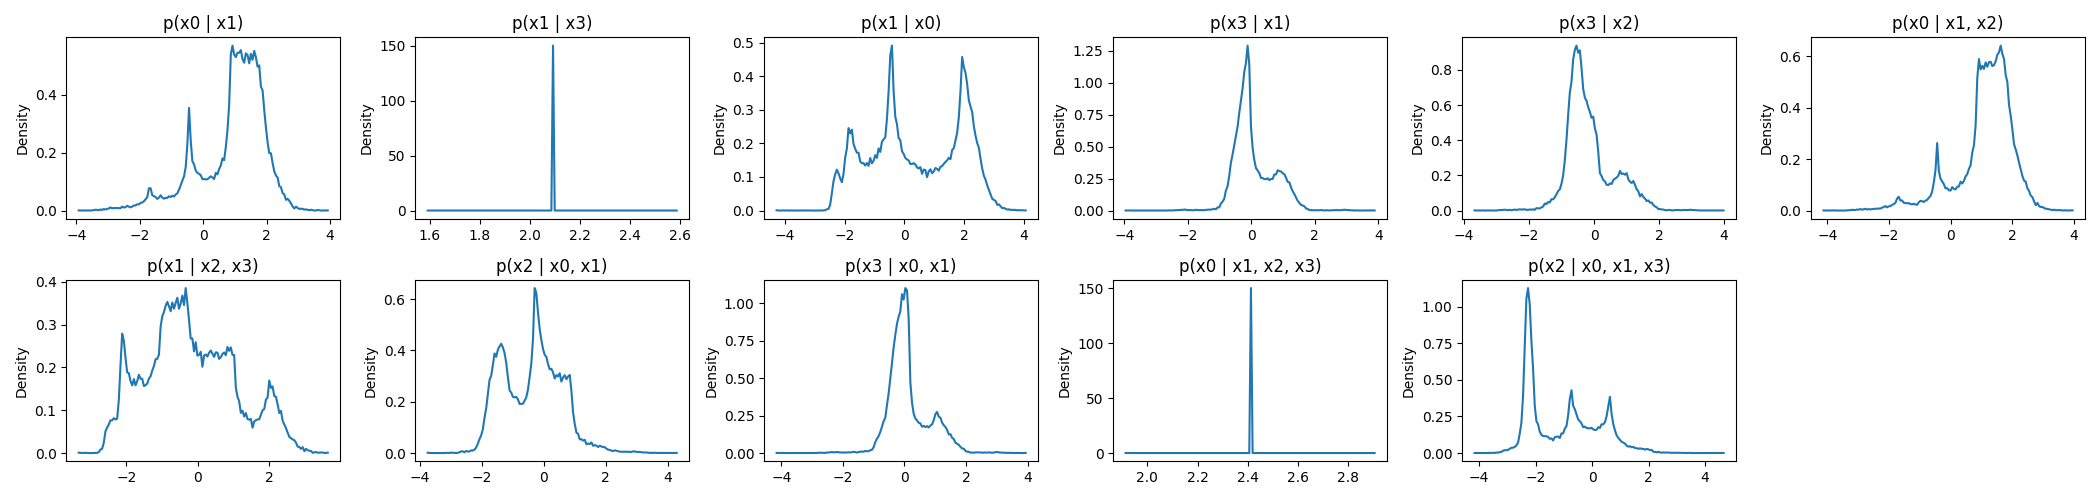
\includegraphics[width=\columnwidth]{images/nonlin-n4-dists.png}
    \caption{An example of a randomly sampled PGM with 4 nodes. Here we plot all the conditional distributions, with one target variable.}
    \label{fig:nonlin-example-pgm-dists}
\end{figure}

\subsubsection{MNIST}

The MNIST benchmark evaluates our framework on real-world image data, providing a practical test of the learned flows on high-dimensional observations. The MNIST dataset consists of 70,000 flattened grayscale handwritten digit images (28$\times$28 pixels, i.e., 784 dimensions) with corresponding labels from 0 to 9.

\paragraph{PGM Structure and Variable Dimensions:}
The MNIST PGM follows a simple causal structure: label $\to$ image, meaning the digit label is the parent of the image data. The variable dimensions are:
\begin{itemize}
    \item \textbf{Image}: 784 dimensions (flattened pixel values, typically normalized to $[0, 1]$)
    \item \textbf{Label}: 10 dimensions (one-hot encoded class labels)
\end{itemize}

\paragraph{Continuous Treatment of Labels:}
While the MNIST labels are inherently categorical (integers from 0 to 9), our flows treat the one-hot encoded label vectors as \textbf{continuous variables}. This easily allows the flow-based models to treat all variables uniformly within the continuous framework.

\paragraph{Dataset Split and Sampling:}
The dataset is partitioned into training (approximately 60,000 samples) and test (approximately 10,000 samples) splits, i.e.\ a 6:1 train/test ratio (the first $6/7$ of the data are used for training). The \texttt{MNISTPGM} class provides conditional sampling via a \texttt{sample()} method:
\begin{itemize}
    \item \textbf{Conditional sampling}: Given a label condition (either as integer index or one-hot encoding), the method samples uniformly from images matching that label within the specified train/test split.
    \item \textbf{Joint sampling}: Without conditions, the method samples both image and label pairs uniformly from the dataset.
\end{itemize}

\subsection{Hyperparameters}
\label{sec:hyperparameters}

Unless otherwise specified, all models (Joint, Static, and Dynamic) were trained using the same budget and optimization settings to ensure a fair comparison.

\begin{table}[h]
\centering
\caption{Hyperparameters used for synthetic PGM benchmarks.}
\begin{tabular}{lr}
\toprule
\textbf{Hyperparameter} & \textbf{Value} \\
\midrule
Optimizer & Adam \\
Initial Learning Rate & $10^{-4}$ \\
Peak Learning Rate & \cam{$10^{-4}$} \\
Ending Learning Rate & \cam{$10^{-6}$} \\
Warmup Steps & 10\% of total \\
Batch Size & \cam{128} \\
Architecture Depth ($D$) & 8 layers \\
\bottomrule
\end{tabular}
\end{table}

\subsection{Baselines}
\label{sec:baselines}

\subsubsection{CAREFL}
We implement Causal Autoregressive Flows (CAREFL) \citep{khemakhem2021causal} as a baseline for structured causal modeling. Unlike the continuous-time ODE flows, CAREFL uses discrete affine transformations. For each node $i$ with parents $pa_i$, the structural equation is:
\begin{equation}
    y_i = g_i(pa_i) \cdot z_i + h_i(pa_i)
\end{equation}
where $z_i \sim \text{Laplace}(0, 1)$ is the noise (following \citealp{khemakhem2021causal} for identifiability), and $g_i, h_i$ are neural networks parameterized to output scaling and shift factors.

\textbf{Implementation:} We use the same \texttt{BlockTriangularStructure} to manage dependencies. The \texttt{log\_prob} is computed by summing the base log-probabilities and the log-determinant terms ($-\sum \log |g_i|$). Sampling is performed by visiting nodes in topological order, computing $g_i, h_i$ from the already sampled parents, and transforming sampled noise $z_i$.

\subsubsection{Guided Baseline}
Our generic baseline is a flow trained on the joint distribution, then conditioned on the required conditions using reconstruction guidance.
The flow is trained on the unconditional joint distribution $p(y)$. During inference, to sample from $p(\Theta | Y_{cond})$, we use reconstruction guidance to steer the ODE trajectories towards the observed values $Y_{cond}$.
\begin{equation}
\mathcal{L}_{rec}(z) = \| z - \hat{z} \|^2 \\
v(z, t) = v_{flow}(z, t) + \gamma \dot\gamma \nabla_{z} \mathcal{L}_{rec}(z)
\end{equation}
where $\gamma$ is from the interpolant noise schedule\cam{, scaled by a guidance strength $\lambda = 7$ (i.e.\ the weight is $-\lambda\gamma\dot\gamma = \lambda(1-t)$ for our interpolant $y_t = t y_1 + (1-t)\epsilon$). This weight is a heuristic: converting a likelihood score into a velocity correction exactly would require the weight $(\alpha^2+\gamma^2)\dot\beta/\beta - (\alpha\dot\alpha + \gamma\dot\gamma) = (1-t)/t$, larger by a factor $1/t$, which diverges at $t=0$ where reconstruction guidance is least accurate. We keep the bounded weight with a tuned strength, as is common for reconstruction guidance}. This method allows for conditional sampling from a model trained only on the joint distribution, but lacks the structural guarantees of our framework.
